\cotefile{83}
\scanpage{145}
\[
 k+k.v+k.w
\]
qui est de rang $3$, et pas égal à $P\ldots$

Je voudrais expliciter tout dans le cas où $H$ et $H'$ sont unipotentes, plus précisément
\[
 H=k\oplus L,\quad H'=k\oplus L'
\]
\margin{i.e. $\unsure{X|H},X'$ sont définis comme les schémas \deleted{\unsure{noy.}}\unsure{aux|vx} de $L\longrightarrow L^{\otimes2}$, $L'\longrightarrow L'^{\otimes2}$ élévation au carré}
\inserted{$P=H\otimes H'=\underbrace{k\oplus L\oplus L'}_{B}+L\otimes L'$}
avec $L,L'$ formés d'éléments de carré nul.

donc \deleted{$\unsure{D|T}_{H,H'}$} $T_{H,H'}$ s'identifie \deleted{\unsure{avec|à}} \inserted{à} $(L\otimes L')^\vee$. \deleted{Choisiss. \unsure{la|base} $u\in L,v\in L'$,} \inserted{La fonction}
\diagram{\begin{tikzcd}[ampersand replacement=\&,row sep=small]
\delta_{H,H'}:\ \& T_{H,H'} \arrow[r] \& \deleted{\unsure{k}}(L\otimes L')^{\otimes-2}\\
\& (L\otimes L')^{-1} \arrow[u,phantom,"\rotatebox{90}{$\simeq$}" description] \arrow[r,Rightarrow,swap,"\substack{\text{élévation}\\\text{\deleted{au} carré}}"] \& (L\otimes L')^{\otimes-2}
\end{tikzcd}}

donc
\[
 H\wedge H'\simeq k\oplus(L\otimes L')
\]
\margin{$L\otimes L'$ formé d'éléments de carré nul}

\deleted{Si $u\in L,v\in L'$}

L'hom
\[
 \deleted{\unsure{H}}X\times_S\deleted{\unsure{H'}}X'\longrightarrow X''=\deleted{\unsure{H}}X\wedge\deleted{\unsure{H}}X'
\]
est donné par
\[
 \underset{\substack{\text{sections}\\\text{de }L,L'\\\text{de carré nul}}}{(\xi,\eta)}
 \longrightarrow
 \underset{\substack{\text{section}\\\text{de }L\otimes L',\\\text{de carré}\\\text{nul}}}{\xi\otimes\eta}
\]
L'hom d'Alg correspondantes
\[
 H\otimes H'\simeq k+L+L'+L\otimes L'\longleftarrow H''=k\oplus L\otimes L'
\]
est celui défini par
% archive sheet number: 144

\scanpage{146}
\uline{NB} On a, \deleted{pour} la structure d'Alg. \inserted{\uline{\unsure{commu|comm.|commut.}}} canonique (produit tens.) sur $P=H\otimes H'$, trois sous-Alg quadratiques
\[
 H,\ H',\ H''
\]
\margin{(où $H''=H\wedge H'$ on suppose maintenant $(2,b,b')k=k$)}
\[
 (P/k\simeq H/\deleted{\unsure{k}}k\oplus H'/k\oplus H''/k\quad\text{comme modules})
\]
et trois involutions \unsure{mutuellt|mutuellement} commutantes
\[
 \sigma_H\deleted{\unsure{=}},\ \sigma_{H'}\quad\text{et}\quad\sigma_{H''}
\]
\margin{($\sigma_{H''}$ défini comme $\sigma_H\sigma_{H'}$)}
de telle façon que
\[
 H=P^{\sigma_H},\quad H'=P^{\sigma_{H'}},\quad H''=P^{\sigma_{H''}}.
\]
\deleted{et que $P$ soit un} \inserted{On a.} $H\cap H'=H'\cap H''=H''\cap H=k$ (\unsure{univ|union}$^{\mathrm t}$), \deleted{\unsure{loc. libre|loc. librement} de rang $4$ et} $P$ est \deleted{engendré} comme algèbre par $H$ et $H'$ (d'où $H\otimes H'\overset{\sim}{\longrightarrow}P$), \deleted{et $\unsure{P|B}$ est aussi} (ce qui caractérise $H''$ comme $H\wedge H'$).

Pour que $P$ soit aussi engendré par $H$ et $H''$ \uline{et} $H'$ et $H''$, il f et s. que $H,H'$ soient étales (et alors $H''$ l'est aussi). Si $H$ est étale, $H'$ non, \inserted{alors $H''$ non plus, et} alors $P$ est engendré par $H,H'$ et $H,H''$ (la relation entre $H'$ et $H''$ p.r. à $H$ est symétrique : $H''\simeq H\wedge H'\iff H'\simeq H\wedge H''$) mais \uline{non} par $H'$ et $H''$. En effet prenant une base $u$ de $\deleted{\unsure{H''}}H$, $v$ de $H'$ avec :
\[
 u^2=u,\ v^2=0\qquad(\text{donc }b=1,\ c=b'=c'=0)
\]
et posant
\[
 w=u\ast v=v-2uv
\]
on aura \deleted{bien} \deleted{\unsure{vw} $w^2=0,\ vw=$} base de $P$
\[
 1,u,v,w
\]
mais on a
\[
 v^2=w^2=vw=0
\]
donc $k[\unsure{w|v}]=H'$ et $k[w]=H''$ engendrent ss-alg
% archive sheet number: 145

\scanpage{147}
\[
 u\mathbin{\otimes_{L,L'}}v\longmapsto u\ast v=-2uv
\]

C'est \unsure{mnt|manift|nul !} injectif comme il se doit, quand $2$ est inv. Par contre, en car. $2$ \deleted{c'est identique} (où les inv. can. sur \deleted{$P$} $H,H',H''$ sont réduites à l'identité !) c'est id nul. Donc $H''$ ne s'identifie pas, alors, à une sous-algèbre de $H\otimes H'$.

Soit $X_L=\operatorname{Spec} k\oplus\underbrace{L}_{\text{carré nul}}$ si
% slanted
\margin{Sans restr. du car.}
donc
\[
 X_L\wedge X_{L'}\simeq X_{L\otimes L'}
\]
% slanted
\margin{Plus \unsure{généralt|généralement}, si \deleted{\unsure{on}} on regarde les quadratiques $X(L,q)$ définis par un mod. inv. $L$ et section $q$ de $L^{\otimes2}$ (comme \unsure{$q^{-1}(0_S)$|$q^{-1}(0)$}), on a \unsure{enc.|fon.} $\deleted{\unsure{H}}X(L,q)\wedge X(L',q')\simeq X(L\otimes L',q\otimes q')$ (iso can.). \unsure{Or|Dz|Du moins} si $2.1_k$ inv. la cat. des sch. quadratiques est \uline{équivalente} à celle des $(L,q)\ldots$}

Ceci montre que les propriétés du produit contracté sont assez différentes des \deleted{produit} \inserted{prop.} familières pour celui des $(\mathbb Z/2\mathbb Z)_S$ torseurs. Ainsi, la donnée
\[
 X_{L''}\simeq\deleted{\unsure{H}}X_L\wedge X_{L'}\qquad\text{i.e.}\ L''\simeq L\otimes L'
\]
n'est pas une donnée sym. en $L,L',L''$, et
\[
 X_L\wedge X_L\simeq\deleted{\unsure{k\oplus}}\unsure{\alpha|X}_{L^{\otimes2}}\simeq k+L^{\otimes2}
\]
n'est pas can. isom. à $(\mathbb Z/2\mathbb Z)_S$ !

[En fait, si $X$ quadratique sur $S$, $X\wedge X$ n'est étale que si $X$ l'est, et alors bien sûr $X\wedge X\simeq(\mathbb Z/2\mathbb Z)_S\ldots$].
% archive sheet number: 146

\scanpage{148}
Il faudrait au moins vérifier\margin{\unsure{!!|!}} l'associativité de l'opération $\wedge$. \deleted{\unsure{Il}} C'est clair si on suppose qu'en les pts de car. $2$, tous les facteurs sauf au plus un sont étales --- mais c'est une condition assez idiote, et sûrement inutile. On \deleted{\unsure{Je|Il}} aimerait une description directe d'un produit contracté multiple de \unsure{var.|rev.} quadratiques
\[
 \bigwedge_{\unsure{j|i}\in I} X_i\qquad I\ \text{ens d'ind. finis}
\]
\deleted{comme \unsure{formes}} comme formes \unsure{multilinéaires|trilinéaires|bilinéaires}. P. ex. sur $H_1,H_2,H_3$ formes \deleted{\unsure{bi}}trilinéaires \deleted{telles} $f(u_1,u_2,u_3)$ telles que
\[
 \begin{aligned}
 f(1,u_2,u_3)&=\operatorname{Tr}u_2)\operatorname{Tr}(u_3)\\
 f(u_1,1,u_3)&=\operatorname{Tr}(u_1)\operatorname{Tr}(u_3)\\
 f(1,u_2,u_3)&=\unsure{\mathrm{Tt}|\mathrm{Tr}}(u_2)\operatorname{Tr}u_3)
 \end{aligned}
\]
(elles forment bien un torseur sous $(L_1\otimes L_2\otimes L_3)^{-1}$), satisfaisant à une condition quadratique convenable --- mais laquelle ??
% archive sheet number: 147

\scanpage{150}
Azumaya rang $4$ \quad (III) \hfill Avril $86$

\figure{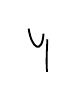
\begin{tikzpicture}[x=0.18cm,y=0.18cm]
\draw[line width=.7pt] (0,2.7) .. controls (.2,1.3) and (.95,.85) .. (1.05,2.35);
\draw[line width=.65pt] (1.32,1.95) .. controls (1.29,1.15) and (1.23,.35) .. (1.3,-.35);
\end{tikzpicture}}
\uline{Digression} sur les produits tensoriels d'espaces affines à involution.

``La donnée, sur un $k$-module $H$ muni d'un élément $1_H$ (``unité'') \inserted{tel que $\lambda\longmapsto\lambda1$ soit injectif de $k$ ds $H$}, d'une \deleted{involution} \inserted{appl. lin.} $x\longrightarrow x'$ qui a) fixe $1_H$ et b) \unsure{induiste|induise|induit} sur $H/k1$ la symétrie, i.e. $x'\equiv-x\bmod k.1$, i.e. $x+x'\in k.1$, équivaut à la donnée d'une forme linéaire $T:H\longrightarrow k$ telle que $T(1_{\unsure{H|.}})=2$, et on aura
% slanted
\margin{i.e. on a une ``coaugmentation'' $k\longrightarrow H$}
\[
 x'=T(x).1-x
\]
\margin{alors $x\longrightarrow x'$ est involutive}

Dualement, \deleted{la donnée} quand on a un $k$-module $E$ et une augmentation
\[
 E\xrightarrow{\varepsilon} k
\]
surjective (ce qui revient à se donner un espace affine \inserted{$A=\varepsilon^{-1}(1)$ sur $k$}, dont le \deleted{\unsure{mo}}module des translations sera $A^0=\operatorname{Ker}(\varepsilon)$), \deleted{revient à se donner un} \inserted{la donnée d'une} involution de $E$ compatible avec $\varepsilon$ (avec id. dans $k$) et induisant sur $A^0=\operatorname{Ker}\varepsilon$ la symétrie $x\longrightarrow-x$, revient à se donner un élément
\[
 t\in E\qquad\text{avec}\qquad\varepsilon(t)=2,
\]
l'involution sera alors
\[
 x\longrightarrow\varepsilon(x)t-x
\]
et $t$ sera fixe. Se donner un espace affine $A$ sur $k$, muni d'un \deleted{\unsure{endo}} \unsure{endom.|involution} qui induise $-\mathrm{id}$ sur le module des translations, revient à se donner un tel syst. (et \deleted{\unsure{l'endom.}} \unsure{autm|élément} est alors involutif).
% archive sheet number: 149

\scanpage{151}
Si $2$ est inv., il y a alors un seul pt fixe dans $A$, et $A$ devient ainsi un module, où l'\unsure{endom|ordinaire} n'est autre que $x\mapsto-x$. Si par contre $2$ est \deleted{inversibl} \inserted{nul} ds $k$, \deleted{\unsure{l'est}} l'élément $t$ est dans le module des translations, et la donnée équivaut à celle de $A$, et de $t\in A^0$ --- et l'involution sera la translation par $t$. Nous nous intéressons cependant aux cas ``à cheval'', tel celui où $k=\mathbb Z$, quand $2$ n'est ni inv., ni nul dans $k$. \deleted{Je veux définir}

Je voudrais définir une opération de produit tensoriel d'espaces affines à involution. \unsure{Soit}\deleted{\unsure{ent}} $(A_1,A_2)$ deux tels espaces, avec involutions $\sigma_1,\sigma_2$ (je laisse tomber la notation $x'$, qui est \unsure{ambigue|ambiguë} \unsure{qqfois|parfois}) et soit $B$ un espace affine sur $k$, les espaces de translation sont notés $A_1^0,A_2^0,B^0$.
% slanted
\margin{il suffit que $B$ soit un \uline{ens.} sur lequel un \deleted{\unsure{groupe}} module $B^0$ opère (\unsure{sans} pt fixe \unsure{et transitif.})}
Une application
\[
 f:A_1\times A_2\longrightarrow B
\]
est dite \deleted{\unsure{une}} $(\sigma_1,\sigma_2)$-bilinéaire, si \deleted{$\unsure{\exists!|\exists}$}
\[
 \deleted{f(x}\quad\exists f^0:A_1^0\times A_2^0\longrightarrow B^0\qquad\text{bil}
\]
% archive sheet number: 150

\scanpage{152}
\unsure{,|1} tel qu'on ait
\[
 \boxed{\left\{\begin{aligned}
 f(x_1+\alpha_1,x_2)&=f(x_1,x_2)+f^0(\alpha_1,\sigma_2x_2-x_2)\\
 f(x_1,x_2+\alpha_2)&=f(x_1,x_2)+f^0(\sigma_1x_1-x_1,\alpha_2)
 \end{aligned}\right.}\tag*{$(*)$}
\]
$\forall\,\alpha_1\in A_1^0,\ \alpha_2\in A_2^0$. On en conclut
\[
 \boxed{\begin{aligned}
 f(x_1+\alpha_1,x_2+\alpha_2)&=f(x_1,x_2)+f^0(\alpha_1,\sigma_2x_2-x_2)+f^0(\sigma_1x_1-x_1,\alpha_1)\\
 &\hspace{8em}-2f^0.(\alpha_1,\alpha_2)
 \end{aligned}}
\]
Si on choisit $x_1,x_2$ comme origines, pour identifier $A_1$ à $A_1^0$ (via les $\alpha_1$) et $A_2$ à $A_{\unsure{3|2}}^0$ (via les $\alpha_2$), posant
\[
 \begin{aligned}
 \sigma_1x_1-x_1&=t_1-2x_1=\tau_1\in A_1^0\\
 \sigma_2x_2-x_2&=t_2-2x_2=\tau_2\in A_2^0
 \end{aligned}
\]
la formule devient
\[
 \underset{\substack{\Vert\,\mathrm{dfn}\\ f(x_1+\alpha_1,x_2+\alpha_2)}}{g(\alpha_1,\alpha_2)}
 =\deleted{\unsure{f(x}}\underset{\substack{\Vert\\ f(x_1,x_2)}}{c}+f^0(\alpha_1,\tau_2)+f^0(\tau_1,\alpha_2)-2f^0(\alpha_1,\alpha_2)
\]
% slanted
\margin{Si $2.1_k=0$, alors $\tau_1=t_1$, $\tau_2=t_2$ sont indép. du choix de $x_1,x_2$, la formule se réduit à $g(\alpha_1,\alpha_2)=c+f^0(\alpha_1,\tau_2)+f^0(\tau_1,\alpha_2)$.}

\deleted{\unsure{Inversement},} Cette formule définit \unsure{entièremt|entièrement} la fonction $g$ \inserted{donc $f$} quand on connaît $c$ ($=f(x_1,x_2)=g(0,0)$), \deleted{\unsure{et}} $\tau_1\in A_1^0,\tau_2\in A_2^0$ (qui définissent les involutions sur $A_1\simeq A_1^0$ \inserted{via $x_1$} et $A_2\simeq A_2^0$ \inserted{via $x_2$} par $\begin{aligned}\alpha_1&\longmapsto\tau_1-\alpha_1\\\alpha_2&\longmapsto\tau_2-\alpha_2\end{aligned}$) et l'application bilin. $f^0$. Quand celle-ci est donnée, on vérifie que la formule précédente définit bien une application $(\sigma_1,\sigma_2)$-bil. Mais si on ne suppose pas $2$ inv., il n'y a aucune
% slanted
\margin{Si $2$ inv., \deleted{\unsure{on}} $\tau_1=0,\tau_2=0$ (en choisissant $x_1,x_2$ fixes par \unsure{$\tau_1,\tau_2$|$\sigma_1,\sigma_2$}), \inserted{via $A_i^0$}, donc $g(\alpha_1,\alpha_2)=-2f^0(\alpha_1,\alpha_2)$ la condition est équiv. à la bilinéarité, sauf sur la const.}
% archive sheet number: 151

\scanpage{153}
garantie que $f^0$ soit connue quand $f$ l'est [Ex : si on prend $\tau^{\prime}=\tau^{\unsure{'|2|\prime\prime}}=0$, $2\,1_k=0$, alors $f$ doit être \uline{constante}]. C'est pourquoi je préfère mettre $f^0$ dans la structure de l'application --- i.e. l'application est un\deleted{\unsure{e}} \deleted{paire}couple
\[
 \begin{aligned}
 (f,f^0):\qquad &f:A_1^{\unsure{1}}\times A_2^{\unsure{2|1}}\longrightarrow B\\
 &f^0:A_1^0\times A_2^0\longrightarrow B^0
 \end{aligned}
\]

On voit tout de suite qu'il y a un accouplement \uline{universel}, dont le module des translations est
\[
 A_1^0\otimes A_2^0
\]
et \deleted{\unsure{qu'on}} on notera $A_1\ast A_2$, espace affine sous $A_1^0\otimes A_2^{\unsure{0|2}}$, avec $(\sigma_1,\sigma_2)$-accouplement
\[
 (x_1,x_2)\longmapsto x_1\ast x_2:\quad A_1\times A_2\longrightarrow A_1\ast A_2.
\]

On peut le réaliser comme sous espace affine de
\[
 E_1\otimes E_2\supset A_1^0\otimes A_2^0
\]
($E_i$ étant le module enveloppant de l'espace affine $A_i$), l'application universelle étant induite par
% archive sheet number: 152

\scanpage{154}
\[
 \boxed{\begin{aligned}
 (x_1,x_2)\longmapsto x_1\ast x_2&=t_1\otimes x_2+x_1\otimes t_2-2x_1\otimes x_2\\
 &=\sigma_1(x_1)\otimes x_2+x_1\otimes\sigma(x_2)
 \end{aligned}}
\]
% slanted
\margin{\uline{NB} Il y a lieu de le prolonger de façon bil. aux modules enveloppants $E_1,E_2$ par $x_1\ast x_2=\underset{\varepsilon(x_1)t_1-x_1}{\underbrace{\sigma_1(x_1)}}\otimes x_2+\deleted{\unsure{\sigma}}x_1\otimes\underset{\varepsilon_2(x_2)t_2-x_2}{\underbrace{\sigma_2(x_2)}}=\varepsilon(x_1)t_1\otimes x_2+\varepsilon(x_2)\unsure{t_2\otimes x_2|x_1\otimes t_2}-2x_1\otimes x_2$.}
on vérifie que sur $A_1^0\times A_2^0$, cette application $f_{A_1^{\unsure{0}},A_2}$, avec
\[
 \begin{aligned}
 f^0_{A_1,A_2}: A_1^0\times A_2^0&\longrightarrow A_1^0\otimes A_2^0\\
 (\alpha_1,\alpha_2)&\longmapsto\alpha_1\otimes\alpha_2
 \end{aligned}
\]

\deleted{\unsure{Ceci}} Bien sûr, $A_1\ast A_2$ est un bifoncteur en $A_1,A_2$. Donc il y a deux involutions $\sigma_1\ast\mathrm{id}_{A_2}$ et $\mathrm{id}_{A_1}\ast\sigma_2$ sur $A_1\ast A_2$, définies par
\[
 x_1\ast x_2\longmapsto\sigma_1(x_1)\ast x_2\qquad
 x_1\ast x_2\longmapsto x_1\ast\sigma_2(\unsure{x_2|\alpha_2})
\]
Je dis qu'elles sont égales, et qu'on a
\[
 \underbrace{\sigma_1(x_1)}_{t_1-x_1}\ast x_2=x_1\ast\underbrace{\sigma_2(x_2)}_{t_2-x_2}=t_1\otimes t_2-x_1\ast x_2
\]
% slanted
\margin{Si $2\,1_k=0$, on a $t_1\otimes t_2\in A_1^0\otimes A_2^0$ ds espace des translations c'est celui qui définit l'inv. can. de $A_1\ast A_2$}
Ainsi, $A_1\ast A_2$ est muni aussi d'une involution \inserted{$\sigma_{A_1\ast A_2}$}. Il est solution du pb universel, cette fois dans les espaces affines involutifs sur $k$, pour les $\sigma$-accouplements d'espaces affines --- où cette fois on met la condition supplémentaire sur $f$
\[
 f(\sigma_1(x_1),x_2)=f(x_1,\sigma_2(x_2))=\sigma_B f(x_1,x_2).
\]
% archive sheet number: 153

\scanpage{155}
Ainsi, $A_1\ast A_2$ est une opération interne dans les espaces affines à involution. Je dis que cette opération a une structure d'associativité, avec \inserted{objet} unité.
% slanted
\margin{il y a une structure de commutativité.}
Ce dernier est l'espace affine trivial $k$ lui-même, avec l'involution $x\longmapsto1-x$, \deleted{\unsure{associée à l'espace}} \inserted{(et non $x\longrightarrow-x$, qui devient triviale en car. $2$ !)}, l'enveloppe affine est $\deleted{\unsure{k\longrightarrow k}}\ k\times k\xrightarrow[\text{somme}]{\varepsilon}k,\quad t_0=(1,1)\mapsto2$.
\inserted{$\sigma_0$ est $(\lambda,\mu)\longmapsto(\mu,\lambda)$}
\margin{$\begin{aligned}k&\hookrightarrow k\times k\\ \lambda&\overset{\mathrm{aff}}{\longmapsto}(\lambda,1-\lambda)\\ k&\overset{\mathrm{lin}}{\hookrightarrow}k\times k\\ \lambda&\longmapsto(\lambda,-\lambda)\end{aligned}$ \inserted{image $A_0=\operatorname{Ker}\unsure{\varepsilon|k}$}}
L'élément $e_0=(\deleted{\unsure{1}}0,1)$ de cet espace affine $A_0$ satisfait
\[
 \sigma_0(e_0)-e_0=1\in k=A_0^0.
\]
Ceci dit, on utilise $e_0$ pour définir une iso. can.
\[
 \begin{aligned}
 A&\overset{\sim}{\longrightarrow} A_0\ast A\deleted{\longrightarrow A}\\
 x&\longmapsto e_0\ast x
 \end{aligned}
\]
compatible avec $A^0\overset{\sim}{\longrightarrow}\underset{\substack{\Vert\\A_0^0}}{k}\otimes A^0$ iso. can.

Pour définir la structure d'associativité, on va définir \unsure{directemt|directement}, pour un nb quelc. de facteurs \inserted{affines involutifs} le produit
\[
 A_1\ast A_2\cdots\ast A_n
\]
% archive sheet number: 154

\scanpage{156}
comme sol. d'un pb universel, que voici : On cherche, pour tt espace affine $B$ sous un \inserted{module} $B^0$, les \inserted{couples} applications $(f,f^0)$
\[
 \begin{aligned}
 f &: A_1\times\cdots\times A_n\longrightarrow B\\
 f^0 &: A_1^0\times\cdots\times A_n^0\longrightarrow B^0
 \end{aligned}
\]
satisfaisant
\[
 \begin{aligned}
 f(x_1,\ldots,x_i+\alpha_i,\ldots x_n)&=f(x_{\unsure{1|0}},\ldots,x_i,\ldots x_n)\\
 &\quad+f^0(\sigma_1x_1-x_1,\ldots,\alpha_{\unsure{1|i}},\ldots\sigma_n\unsure{a_n|x_n}-x_n)
 \end{aligned}
\]
pour tt $i\in\{1,\ldots,n\}$ et $\alpha_i\in A_i^0$. Sauf erreur, la solution du pb universel se réalise comme sous espace affine de
\[
 E_1\otimes\cdots\otimes E_n
\]
sous
\[
 E_1^0\otimes\cdots\otimes E_n^0
\]
formé$^*$ par les éléments
% slanted
\margin{$^*$ non, \uline{engendré}, pas ``formé'', cf cas \unsure{où} $2\,1_k=0$ et tous les $t_i$ sont nuls (alors $\ast x_i=0$ identiquement !)}
\[
 x_1\ast x_2\ast\cdots\ast x_n\qquad(\text{pour }x_i\in A_i)
\]
définis ainsi
\[
 \begin{aligned}
 x_1\ast x_2\cdots\ast x_n={}&\left(\sum t_1\cdots t_{n-1}x_n\right)\deleted{\unsure{=|-}}-2\left(\sum t_1\cdots t_{n-2}x_{n-1}x_n\right)+4\left(\sum t_1\cdots t_{n-3}x_{n-2}x_{n-1}x_n\right)\\
 &\ldots+(-1)^{n+1}2^{n-1}x_1x_2\cdots x_n .
 \end{aligned}
\]
% slanted
\margin{Pour un accouplement multilinéaire des $E_i$, en remplaçant $t_i$ par $\varepsilon_i(x_i)t_i$}

Quand on change l'\uuline{un} des $x_i$ en $\sigma_i(x_i)=t_i-x_i$, le produit est changé en
\[
 t_1t_2\cdots t_n-x_1\ast x_2\ast\cdots\ast x_n.
\]
% archive sheet number: 155

\scanpage{157}
On peut prolonger \deleted{\unsure{bi}}multilinéairement en une application
\[
 \begin{aligned}
 E_1\times\cdots\times E_n&\mathbin{\unsure{\text{---}|\longrightarrow}} E_1\otimes\cdots\otimes E_n\\
 (x_1,\ldots x_n)&\longmapsto x_1\ast x_2\cdots\ast x_n
 \end{aligned}
\]
donné par
\[
 \mathop{\ast}_{i}x_i=\sum_{i=1}^{n}(-1)^{i\unsure{+|-}1}2^{i-1}
 \biggl(\sum\underbrace{\varepsilon_1(x_1)t_1\varepsilon_2(x_2)t_2\cdots\varepsilon_{n-i}(x_{n-i})t_{n-i}}_{\substack{n-i\ \text{facteurs}\\\varepsilon(x_j)t_j}}
 \underbrace{x_{n-i+1}\cdots x_n}_{i\ \text{facteurs }x}.
\]
Dont l'image est le sous-module de $\bigotimes E_i$ engendré par $\mathop{\ast}A_i$. Ce sous module \deleted{est} contient \inserted{donc} $\bigotimes A_i^0$ \inserted{et $t_1t_2\cdots t_n$}, et son quotient par $\bigotimes A_i^0$ est monogène, \deleted{et engendré par $t_1\cdots t_n$ (?).}
% slanted
\margin{vérifier \unsure{si un pb|ce qui se passe} en car $2$ !}

Formule plus jolie en termes des $\sigma_i$
\[
 \begin{aligned}
 x_1\ast x_2\cdots\ast x_n
 &=\sum_{\substack{i\ \text{impair}\\1\leq i\leq n}}\quad\sum_{\binom ni\text{ termes}}
 x_1\cdots x_i\,\sigma_{i+1}(x_{\unsure{i-1|i+1}})\cdots\sigma_n(x_n)
 &&(2^{n-1}\text{ termes})\\
 \sigma(x_1\ast\cdots\ast x_n)
 &=\sum_{\substack{i\ \text{pair}\\0\leq i\leq n}}\quad\sum_{\binom ni\text{ termes}}
 x_1\cdots x_i\,\sigma_{i+1}(x_{\unsure{i-1|i+1}})\cdots\sigma_n(x_n)
 &&(2^{n-1}\text{ termes})\\
 (x_1\ast\cdots\ast x_n)+\sigma(x_1\ast\cdots\ast x_n)
 &=t_1t_2\cdots t_n\,\varepsilon_1(x_1)\varepsilon_2(x_2)\cdots\varepsilon_n(x_n)
 \end{aligned}
\]
On a
\[
 (\deleted{\unsure{x_1+}}\alpha_1)\ast x_2\cdots\ast x_n=\inserted{\deleted{\unsure{x_1\ast x_2\cdots\ast x_n+}}}\alpha_1\otimes(\sigma_2(x_2)\deleted{\unsure{+}}-x_2)\otimes\cdots\otimes(\sigma_n(x_n)-x_n)
\]
si $\alpha_1\in E_1^0$ et $n-1$ formules similaires.

Si $2$ est inversible, alors $t_1\otimes\cdots\otimes t_n$ est la base d'un supplémentaire canonique de $\bigotimes A_i^0$ dans le sous-module \inserted{$E$} de $\bigotimes \deleted{\unsure{A}}E_i$ engendré par $\mathop{\ast}_i A_i$. On peut alors
% archive sheet number: 156

\scanpage{158}
considérer $E$ comme le module enveloppant de $\mathop{\ast}A_i$, en le munissant de l'augmentation
\[
 \varepsilon:E\longrightarrow k
\]
définie par
\[
 \varepsilon(\underbrace{t_1t_2\cdots t_n}_{t})=2
\]
On notera que $\varepsilon$ n'\uline{est pas} induit par
\[
 \deleted{\unsure{\varphi}}\varepsilon_1\otimes\cdots\otimes\varepsilon_n:\bigotimes E_i\mathbin{\unsure{\text{---}|\longrightarrow}}k
\]
qui transforme $t_1t_2\cdots t_n$ non pas en \unsure{$2$}, mais en $2^n$.

Le groupe $(\mathbb Z/2\mathbb Z)^n$ opère sur $P=\bigotimes E_i$ via les $\sigma_i$, et les différents caractères définissent des sous-modules propres, dont $\bigotimes E_i$ est la somme directe (si $2$ inv !). Un car. est donné par $\alpha=(\alpha_1,\ldots,\alpha_n)\in(\mathbb Z/2\mathbb Z)^n$, et \deleted{\unsure{son}}
\[
 P_\alpha=\{x\in P\mid \sigma_1^{\deleted{\unsure{\alpha_1}}\beta_1}\otimes\cdots\otimes\sigma_n^{\deleted{\unsure{\alpha_n}}\beta_n}(x)=(-1)^{\alpha_1\beta_1+\alpha_2\beta_2\cdots+\alpha_n\beta_n}x\}
\]
\margin{$\forall$ syst. d'entiers $\beta_i$ mod \uline{$2$}}
Ceci dit, $E$ est le sous espace propre associé au caractère somme $\alpha=(1,\ldots,1)$ i.e.
\[
 E=P_{1,\ldots,1}=\{x\in P\mid(\sigma_1^{\beta_1}\deleted{\unsure{\otimes\sigma}}\otimes\cdots\otimes\sigma_n^{\beta_n})x_n)=(-1)^{\sum\beta_i}x\}
\]
% archive sheet number: 157

\scanpage{159}
Finalement, on trouve des formules plus jolies en éliminant les $t_i$ et $\varepsilon_i$, et en ne travaillant qu'avec les $\sigma_i$. Cela nous amène à un contexte différent : celui des \deleted{\unsure{var.}} modules \inserted{involutifs (i.e. modules} munis d'une involution). \unsure{Éventuellemt|Éventuellement}, on se donne dans $E_i$ un sous-module $E_i^0$, de telle façon que $\sigma_i$ soit $-\mathrm{id}_{E_i^0}$ sur $E_i^0$, et soit id sur $E_i/E_i^0$ (cet $E_i^0$ est \deleted{\unsure{g}} unique \deleted{\unsure{s}} si $2$ inv., alors c'est le sous-module propre $E_i^-$, formé des \unsure{à|$x$} tels que $\sigma_i x=-x$) Un \uline{accouplement involutif} \deleted{\unsure{de ces|de}} \inserted{vers} un module $E$, sera une application multilinéaire
\diagram{\begin{tikzcd}[ampersand replacement=\&,row sep=small]
\deleted{\unsure{F}}E_1\times\cdots\times E_n\arrow[r,"f"] \& E\quad\text{munie de}\\
\deleted{\unsure{f^0:f}}\ E_1^0\times\cdots\unsure{+|\times} E_n^0\arrow[ur,"f^0"'] \&
\end{tikzcd}}
satisfaisant les relations de la forme
\[
 \begin{aligned}
 f(x_1+\alpha_1,x_2\ldots \unsure{a_n|x_n})&=f(x_1,\ldots x_n)+f^0(\alpha_1,\sigma_2(x_2)-x_2,\\
 &\hspace{12em}\ldots\sigma_n(x_n)-x_n)
 \end{aligned}
\]
pour $\alpha_1\in E_1^0$ (et les $n-1$ autres relations similaires)

On aura donc
\[
 f(\alpha_1,\alpha_2\ldots\alpha_n)=(-2)^{n-1}f^0(\alpha_1,\alpha_2,\ldots\alpha_n)
\]
% archive sheet number: 158

\scanpage{160}
La solution du pb \inserted{\unsure{ci-dessus|semi-linéaire}$^{*}$} universel est un module quotient de $\bigotimes E_i^0\oplus\bigotimes E_i$, c'est une extension de $\bigotimes E_i/E_i^0$ par $\bigotimes E_i^0$ :
\[
0\longrightarrow\bigotimes E_i^0\xrightarrow{i}\mathop{*}_{i}(E_i,\sigma_i)^{\deleted{\unsure{0|\wedge}}}\xrightarrow{j}\bigotimes(E_i/E_i^0)\longrightarrow0
\]
% slanted
\margin{attention, ce n'est peut-être vrai tel \unsure{quel|que} si on suppose p. ex. \unsure{que} $E_i/E_i^0$ \unsure{et} $E_i^0$ \unsure{plat. des|plats. des} extensions convenablement \unsure{scindées|scindée} et $2$ inv.}
% slanted
\margin{NB On devrait écrire $E_i^-$ al d $E_i^0$ et $E_i^+$ al d $E_i/E_i^0$}

Quand on a des isos $E_i/E_i^0\simeq k$ alors $\mathop{*}_{i}(E_i,\sigma_i)$ apparait comme une extension de \deleted{$k$}$k$ par $\bigotimes E_i^0$ -- on retrouve le contexte des espaces affines.
% slanted
\margin{$*$ \deleted{En effet,} Car on a si \deleted{deux parmi les $\sigma_i$ sont $\sigma_i$} \deleted{sont} $\sigma_i=\mathrm{id}$, alors \deleted{$j$ est iso, alors} \deleted{\unsure{nul}!} $\mathop{\unsure{*|\bigotimes}}_{i}(E_i,\sigma_i)\simeq\bigotimes E_i/E_i^0\oplus\bigotimes E_i^0$ et $i$ est quand même injectif}

On a toujours un hom canonique
\[
\mathop{*}_{i}(E_i,\sigma_i)\xrightarrow{\tau}\bigotimes E_i
\]
donné par la formule devinée tantôt (pour $n=2$, c'est la formule
\[
x_1*x_2=\sigma_1 x_1\otimes x_2+x_1\otimes\sigma_2 x_2\qquad)
\]
mais on a
\diagram{\begin{tikzcd}[ampersand replacement=\&,column sep=large]
\bigotimes E_i^0 \arrow[d,"i"'] \arrow[dr,"{(-2)^{n-1}\mathrm{can}}"] \& \\
\mathop{*}(E_i,\sigma_i) \arrow[r,"\tau"] \arrow[dr,"{2^{n-1}j}"'] \& \bigotimes E_i \arrow[d,"\mathrm{can}"]\\
\& \bigotimes E_i/E_i^0
\end{tikzcd}}
% slanted
\margin{finalement, cette application $\tau$ n'est pas tellement utile, je crois, si $2$ n'est pas supposé inversible.}
C'est donc inj. si $2$ inv., mais pas en général.

On a là une loi de composition \inserted{interne} associative, commutative,
% archive sheet number: 159

\scanpage{161}
Si $2$ inv., la catégorie des modules à involution équivaut à celle des \deleted{\unsure{paire|paires}} couples de modules $(\underset{\substack{\shortparallel\\ E^0}}{E^-},E^+)$, et l'opération $*$ est l'opération de produit tensoriel séparément sur les deux facteurs \deleted{\unsure{linéaires|linéaire}} -- aucun mystère ! L'opération est délicate et utile, par contre, si $2$ non inversible. (p. ex. en car. $2$)

\begin{center}\rule{1.8em}{0.4pt}\end{center}

Revenons au contexte des espaces affines. Si on a un espace affine $A$ sous un module de translations \uline{inversible} \inserted{$L=A^0$}, alors la donnée d'un diviseur quadratique dans $\check{\mathbb V}(A)$ (le schéma \deleted{\unsure{espace}} \inserted{torseur sous $\check{\mathbb V}(A^0)$} défini par $A$) revient à la donnée d'une forme quadratique sur $E$ (enveloppe affine de $A$) à valeurs dans $L^{\otimes2}$
\[
q_E:E\longrightarrow L^{\otimes2}
\]
(i.e. d'une ``fonction \deleted{\unsure{pol.|polyn.}} \inserted{$q_A$} de degré $\leq2$ sur $A$''), telle que $q_L=q\mid L$ (la ``partie hom de $q$'') soit \deleted{\unsure{l'élem|l'élévation}} \deleted{forme} quadr. can
\[
L\longrightarrow L^{\otimes2}\qquad u\longmapsto u^{\otimes2}
\]
% archive sheet number: 160

